\chapter{Object Recognition}
\paragraph{} When the certain object is selected on the left picture, the same object on the right picture has to be automatically located. Let the square matrix $I_{L}$ represent selected object on the left picture. Knowing the properties of stereoscopic pictures (the objects are horizontally shifted), we can define search area within the right picture – matrix $I_{R}$.
Vertical dimensions of $I_{R}$ and $I_{L}$ should be the same, while horizontal dimension of $I_{R}$ should be higher.

\paragraph{}Our next step is to find the location within the search area IR, where the picture best fits matrix $I_{L}$. We do that by subtracting matrix $I_{L}$ from all possible submatrixes (in size of matrix $I_{L}$) within the matrix $I_{R}$. When size of the matrix IL is NxN and size of the matrix $I_{R}$ is $MxN$, where $M>N$, $M-N+1$ submatrixes have to be checked.

\begin{figure}[H]
	\centering
	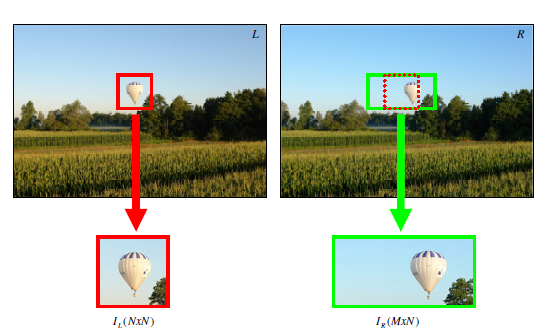
\includegraphics[height= 8cm, width= 14cm]{project/images/y.png}
	\caption{\textsc{Selected object on left picture and search area on right picture.}}
\end{figure}
\paragraph{}The result of each subtraction is another matrix Ii which tells us how similar subtracted images are. More similar two subtracted images are, lower is the mean absolute value of matrix $I_{i}$.\\
\paragraph{} Images in the first example do not match, while in the second example images match almost perfectly.

\paragraph{} The matrix $I_{K}$ with the lowest mean of its elements, represents the location where matrix $I_{L}$ best fits to matrix $I_{R}$. This is also the location of the chosen object within the right image. Knowing the location of the object in the left and right image allow us to calculate the distance between the pictures:\\

\begin{equation}
x_{L}-x_{D}=\frac{N}{2}+K-1-\frac{M}{2}
\end{equation}\\

The distance $(x_{L}-x_{D})$ is the most vital and a bit complex in calculation. This value determines the amount of match between frames captured from both cameras.
Rest of the values are pre-defined and constant, the only value varying is $(x_{L}-x_{D})$. Our work is in finding this value and in turn calculating value of D, which gives the depth.
